%Chapter{Sintesis de óxido de grafeno}
El método de síntesis empleado en esta tesis es el propuesto por Abdolhosseinzadeh \citep{Abdolhosseinzadeh2015}, que se basa en la ruta de síntesis propuesta por Hummers para el óxido de grafito. La principal diferencia entre ambos es que Abdolhosseinzadeh introduce etapas de sonicación, para asistir en la exfoliación del óxido de grafito.

En una síntesis normal, 1 g de grafito en polvo (Sigma-Aldrich $>$99\%) o en hojuelas (Superior Graphite $>$80\%), es depositado en 50 ml de ácido sulfúrico (\ce{H_2SO_4}, Baker 97.8\%) en un vaso precipitado de 250 ml, el cual debe ser enfriado en un baño de hielo con agitador magnético, para mantener la mezcla a una temperatura inferior a 10 \degree C. Una vez el grafito se ha dispersado en el ácido sulfúrico, se agregan lentamente 3 g de permanganato de potasio (\ce{KMnO_4}, Chemix 99.44\%), asegurando mantener la temperatura de la mezcla bajo los 10 C y así evitar la explosión del heptaóxido de manganeso (\ce{M2O7}),\citep{Dreyer2010}. Luego de 15 minutos de agitación, se remueve el baño de hielo y la mezcla es agitada por 25 minutos a temperatura ambiente, seguido de 5 minutos en un baño ultrasónico (99\% de potencia, SB-3200DTD Ultrasonic Cleaner). Este proceso de agitación-sonicación es repetido 12 veces, alcanzando un total de 6 horas en completarse. Una vez finalizado el proceso, se agregan rápidamente 200 ml de agua destilada, produciendo una reacción exotérmica que genera subproductos gaseosos. La dispersión se vuelve marrón, color característico del óxido de grafeno. Posteriormente, la solución se divide en dos partes iguales que deben sonicarse por dos horas más. Una de las partes es reducida, proceso que será explicado más adelante, mientras la otra es tratada con agua oxigenada (\ce{H_{2}O_2}), tal como lo menciona Hummers en su escrito original, con la finalidad de reducir el permanganato y dióxido de manganato restante en la solución. Para esto se añaden 20 ml de \ce{H_2O_2} al 30\% lentamente bajo agitación constante. La solución se vuelve de color amarillo brillante y libera gases. Cuando la evolución de gases cesa, se remueve del agitador magnético y se deja a temperatura ambiente. Transcurrido un día de reposo, el material precipita al fondo del vaso, se remueve el resto de la solución acuosa y se rellena el vaso con agua destilada. Este proceso de lavado es realizado al menos cuatro veces. Posteriormente se remueve la mayor cantidad de agua posible y se deja secar a temperatura ambiente.

\begin{figure}
	\centering
	\fbox{
		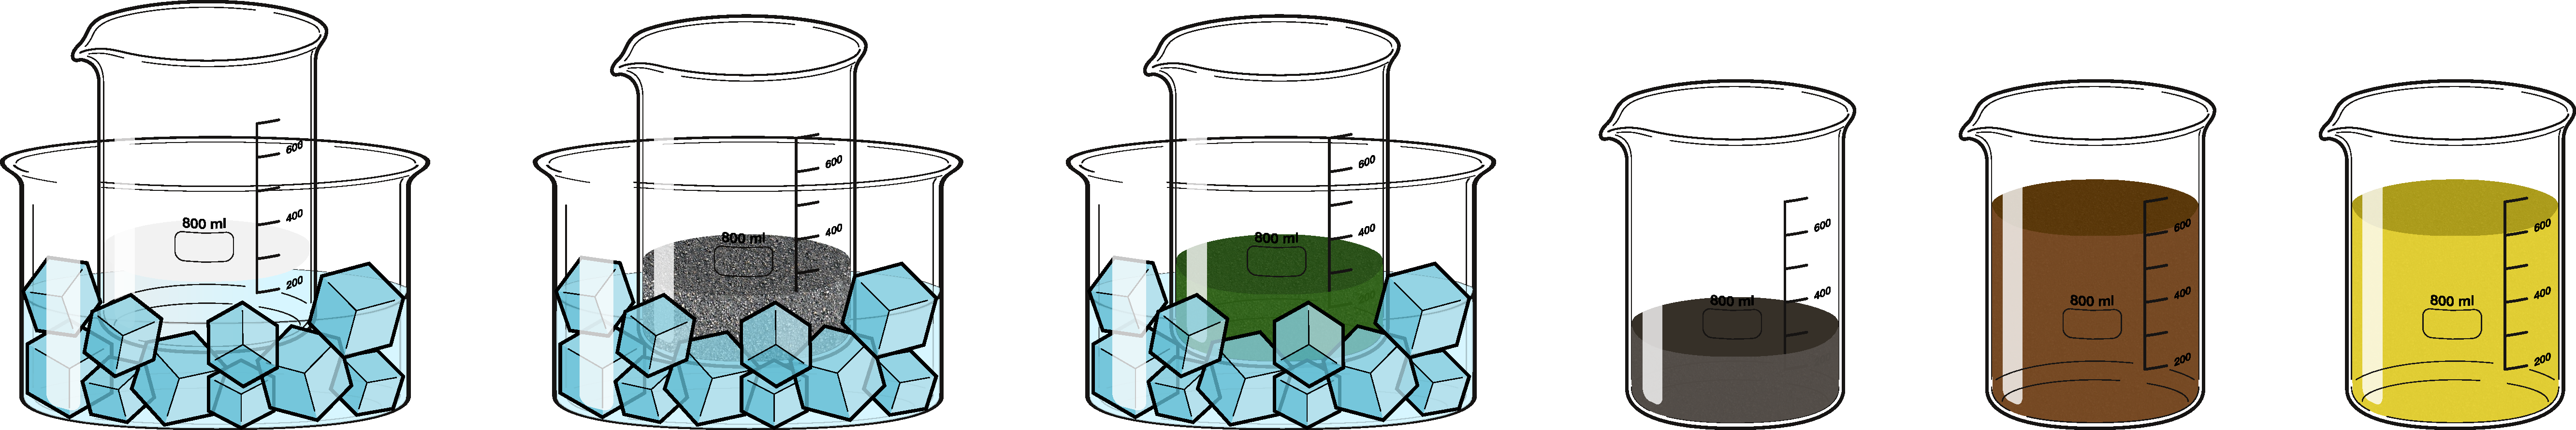
\includegraphics[width=1.4\textwidth]{experimental_method_GO.pdf}
	}
	\caption[Método experimental para la síntesis de óxido de grafeno]{Método experimental para la síntesis de óxido de grafeno.}
\end{figure}


